%!TEX root = ../tesis.tex
 \chapter{Tecnolog\'ias y Herramientas}
\label{sec:tecnologias}

En la actualidad existe un gran n\'umero de herramientas de software que pueden utilizarse para la implementaci\'on de un
sistema de reconocimiento del habla. Si bien esta diversidad representa una ventaja, esto requiere
la selecci\'on de la tecnolog{\'\i}a adecuada. Es selecci\'on conforma la primera tarea a llevar a
cabo por las personas que deseen trabajar en esta \'area.

Este cap{\'\i}tulo presenta, categoriza y eval\'ua varias alternativas tecnolog{\'\i}cas disponibles, relacionadas
al reconocimiento del habla, con el fin de facilitar la elecci\'on de la herramienta adecuada
de acuerdo a las necesidades de cada caso. La siguiente clasificaci\'on y criterios que ser\'an presentados son
una propuesta que forma parte de este trabajo de grado.

Inicialmente, se clasifican las herramientas en las siguientes categor{\'\i}as:
\begin{itemize}
	\item Aplicaciones: herramientas software que permiten al usuario realizar una o
	varias tareas \mbox{espec{\'\i}fic as \cite{GoodwillComputer}}.
    \item \gls{api}: interfaces entre una base de c\'odigo y
	el programador \cite{DoucetteOnApi}. Esta abstracci\'on puede verse como una caja negra
	(los detalles de la implementaci\'on se mantienen ocultos) que provee una determinada funcionalidad.
	\item Librer{\'\i}as/Frameworks: con junto de m\'etodos o funciones a los que se puede invocar.
	En el caso de un framework, incluye tambi\'en patrones de dise\~no
	\mbox{predefinidos \cite{FowlerInversion}}.
\end{itemize}

Las categor{\'\i}as citadas anteriormente representan, diferentes enfoques para realizar el trabajo
de reconocimiento del habla. A modo de discernir entre los mismos, se establecen
los siguientes criterios generales de evaluaci\'on:
\begin{itemize}
	\item Conocimiento t\'ecnico necesario: nivel de conocimiento relativo al \'area necesario para la
	utilizaci\'on de la herramienta. 
	\item Productividad: raz\'on entre las funcionalidades que pueden implementarse,o tareas que pueden
	realizarse, utilizando la herramienta y recursos que toma la implementaci\'on.
	\item Flexibilidad: facilidad de adaptaci\'on de la herramienta para la soluci\'on de diferentes
	tipos de problemas.
\end{itemize}

La siguiente figura presenta de forma esquematizada el contenido del cap{\'\i}tulo, y puede tomarse como
gu\'ia para la lectura de las secciones del mismo.

\begin{figure}[H]
\centering
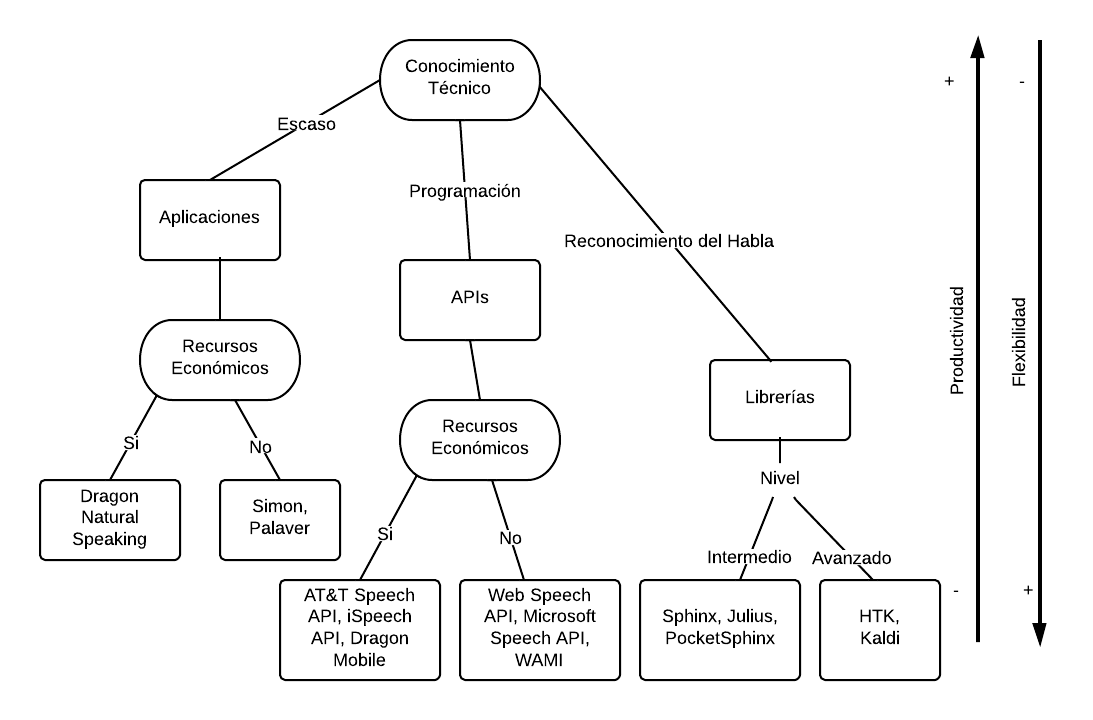
\includegraphics[width=1\linewidth]{./graphics/esquema-herramientas.png}
\caption{Esquema que presenta el contenido del cap\'itulo}
\label{figure:esquema-herramientas}
\end{figure}

\section{Aplicaciones}
\label{sec:aplicaciones}

% introduccion

Las soluciones de reconocimiento del habla, catalogadas como aplicaciones, propocionan
a los usuarios finales los medios necesarios para realizar determinadas tareas mediante
la voz: dictado autom\'atico, navegaci\'on de interfaces, etc\'etera; sin
la necesidad de tener un conocimiento previo de los conceptos relacionados al
reconocimiento del habla. \'Estas aplicaciones presentan las siguientes 
caracter\'isticas en cuanto a los criterios generales de evaluaci\'on:

\begin{itemize}
    \item Conocimiento t\'ecnico: requieren de poco conocimiento t\'ecnico debido a que \'estas
        soluciones se ofrecen como un producto a los usuarios finales, por lo tanto, sus funcionalidades
        pueden utilizarse directamente sin necesidad de entender los componentes que intervienen
         en el sistema.
    \item Productividad: teniendo en cuenta el criterio anterior, cabe resaltar que con
        las aplicaciones se puede lograr un buen grado de productividad, porque los esfuerzos
        de los usuarios se enfocan en realizar determinadas tareas utilizando las funcionalidades
         disponibles.
    \item Flexibilidad: la flexibilidad para esta categor\'ia de soluciones es reducida, porque las
        funcionalidades que ofrece cada aplicaci\'on se encuentran orientadas a resolver tareas
        espec\'ificas: dictado autom\'atico, para la transcripci\'on de documentos; reconocimiento
        de comandos, para navegar interfaces; reconocimiento del habla, para 
        automatizaci\'on de servicios de operador. Cada aplicaci\'on tiene un \'ambito de aplicabilidad
        lo cual impone un l\'imite en su flexibilidad, en comparaci\'on a otras categor\'ias que
         se ver\'an m\'as adelante.
\end{itemize}

\subsection{Criterios Espec\'ificos de Evaluaci\'on}

Los criterios espec\'ificos nos permiten evaluar a las aplicaciones en cuanto a factores
particulares y relevantes para esta categor\'ia. A continuaci\'on se presentan los criterios 
espec\'ificos de evaluaci\'on para las aplicaciones:

\begin{itemize}
    \item Precio
    \item Soporte para m\'ultiples idiomas
\end{itemize}

\subsection{Ejemplos de Aplicaciones}

\subsubsection{Simon}
\label{sec:simon}

\emph{Simon} es un programa de reconocimiento del habla de c\'odigo abierto que tiene como objetivo
reemplazar el teclado y mouse \cite{SimonListen}. Esta dise\~nado para ser muy flexible y permite la
personalizaci\'on para cualquier aplicaci\'on que necesite incorporar reconocimiento
del habla. Adem\'as, \'este programa pretende ayudar a personas con alguna discapacidad, debido
a que busca brindarles la posibilidad de escribir correos electr\'onicos, navegar internet, etc.

\begin{itemize}
    \item \emph{Precio:} esta herramienta es gratuita y de c\'odigo abierto.
    \item \emph{Soporte para m\'ultiples idiomas:} \emph{Simon} es una herramienta independiente del idioma,
    debido a que permite incorporar nuevos modelos estad\'isticos. Si se desea
	utilizar el espa\~nol, por ejemplo, simplemente hay que incorporar el modelo estad\'istico que representa
    a los sonidos que forman las palabras de dicho idioma.
    \item \emph{Facilidad de configuraci\'on:} esta herramienta est\'a dise\~nada para que sea
	f\'acilmente configurable desde su interfaz gr\'afica. Utiliza el concepto de Escenarios para identificar a un contexto (aplicaci\'on)
	que se desea operar a trav\'es de la voz. Brinda, por defecto, un modelo base para el idioma ingl\'es (el
    modelo prove\'ido por Voxforge\cite{Voxforge}), pero permite incorporar otros modelos e incluso generar nuevos.
    \item \emph{Soporte para dispositivos m\'oviles:} \emph{Simone} es un cliente de Simon para dispositivos m\'oviles. Aunque las
	capacidades de este cliente son limitadas, actualmente permite: controlar una computadora a trav\'es de una red
	local inal\'ambrica (utilizar el tel\'efono como micr\'ofono), realizar llamadas a contactos y navegar el software. 
    La versi\'on inicial de \emph{Simone} se desarroll\'o para 
	Meego\footnote{Meego fue un sistema operativo de c\'odigo abierto que result\'o de la uni\'on de
	los sistemas operativos \emph{Maemo} de Nokia y \emph{Moblin} de Intel, con la intenci\'on de competir
	con el sistema operativo \emph{Android} de Google.}, aunque el soporte para Android se encuentra en desarrollo.

\end{itemize}

\subsubsection{Palaver}
\label{sec:palaver}

\emph{Palaver} es una aplicaci\'on, actualmente disponible solo para Linux orientada principalmente
al control de funcionalidades de las computadoras a trav\'es de la voz, aunque tambi\'en
puede utilizarse para transcripci\'on \cite{Palaver}. \emph{Palaver} utiliza un diccionario para
definir los comandos que soporta y, adem\'as, permite definir nuevos comandos a trav\'es
de un sistema de \foreign{plugins}.

\begin{itemize}
    \item \emph{Precio:} esta herramienta es gratuita y de c\'odigo abierto.
    \item \emph{Soporte para m\'ultiples idiomas:} esta herramienta delega la interpretaci\'on de
	la voz a los servidores de Google, por lo tanto, es posible utilizar \emph{Palaver} en otros idiomas.
    Sin embargo, esto implica la modificaci\'on del diccionario de comandos, ya que por 
    defecto \emph{Palaver} provee un diccionario para el idioma ingl\'es. Adem\'as, al delegar el
    reconocimiento a servidores externos, es necesario tener conexi\'on a internet para utilizar
    esta herramienta.
    \item \emph{Facilidad de configuraci\'on:} esta herramienta permite extender los comandos soportados a 
    trav\'es de un sistema de plugins, adem\'as es posible configurar otros aspectos de la aplicaci\'on
    (como el idioma). 
    Sin embargo, no existe una interfaz gr\'afica para realizar las configuraciones, lo que reduce en
    cierta medida la facilidad de configuraci\'on.
    \item \emph{Soporte para dispositivos m\'oviles:} actualmente esta herramienta no ofrece soporte
    para dispositivos m\'oviles.
\end{itemize}

\subsubsection{Dragon Naturally Speaking}
\label{sec:nuance}

\foreign{Dragon Naturally Speaking} es una aplicaci\'on de la empresa \emph{Nuance Communications} 
que permite interactuar con las computadoras a trav\'es de la voz \cite{DragonNaturallySpeaking}. Permite
crear documentos, escribir correos electr\'onicos, lanzar aplicaciones, abrir archivos, controlar
el mouse, etc. Esta herramienta presenta una interfaz de usuario minimalista y posee tres
\'areas principales de aplicaci\'on: dictado, s\'intesis de habla y reconocimiento de comandos. 
El usuario puede dictar y obtener la transcripci\'on del habla en forma de texto escrito, obtener
una versi\'on sintetizada de un documento como un flujo de audio, y emitir comandos de voz que
son reconocidos por el sistema.

\begin{itemize}
    \item \emph{Precio:} esta herramienta viene en varias ediciones, la \foreign{Home Edition} se puede
        obtener desde \$99.99 y la versi\'on \foreign{Premium} desde \$199.99
    \item \emph{Soporte para m\'ultiples idiomas:} este programa soporta los siguientes idiomas: Ingl\'es, Franc\'es,
	Alem\'an, Espa\~nol, Italiano, Holand\'es. Adem\'as cabe destacar que esta herramienta soporta 
    m\'ultiples acentos.
    \item \emph{Facilidad de configuraci\'on:} esta herramienta presenta una interfaz minimalista a 
    trav\'es de la cual se puede modificar la configuraci\'on del sistema.
    \item \emph{Soporte para dispositivos m\'oviles:} \foreign{Dragon Remote Mic} es una aplicaci\'on para 
    \emph{iOS} y \emph{Android} que permite convertir un tel\'efono celular en un microfono inal\'ambrico 
    para el sistema. Adem\'as, la empresa \foreign{Nuance Communications} proporciona otros productos, 
    derivados de \foreign{Dragon}, orientados a dispositivos m\'oviles.
\end{itemize}


%!TEX root = ../../tesis.tex
\section{Interfaces de Programaci\'on de Aplicaciones}
\label{apis}

% introduccion

Una interfaz de programaci\'on de aplicaciones (tambi\'en conocida como \gls{api} por sus siglas 
en ingl\'es) proporciona a los desarrolladores los medios necesarios para integrar funcionalidades de
reconocimiento del habla al \foreign{software} que implementan, sin necesidad de poseer
conocimiento en detalle del \'area. De acuerdo a los criterios de evaluaci\'on generales, 
pueden mencionarse las siguientes caracter{\'\i}sticas:

\begin{itemize}
 	\item Conocimiento t\'ecnico necesario: aunque no requieren conocimiento sobre detalles de implementaci\'on
 	del \'area de reconocimiento del habla, si resultan necesarios conocimientos b\'asicos de
 	programaci\'on, por lo cual resulta inadecuada su utilizaci\'on por parte de usuarios finales.
 	\item Productividad: la utilizaci\'on de una interfaz de programaci\'on de aplicaciones permite
 	al desarrollador abstraerse de la complejidad subyacente del problema, lo cual resulta en
 	un alto grado de productividad. Sin embargo, el ocultamiento de los detalles del proceso
 	puede ser un factor negativo en algunos \'ambitos, como el \mbox{acad\'emico}.
 	\item Flexibilidad: estas herramientas presentan un buen grado de flexibilidad, debido a
 	que no est\'an orientadas a una tarea en particular. La selecci\'on del problema espec{\'\i}fico
 	que se soluciona utilizando reconocimiento del habla es responsabilidad del desarrollador
 	que utiliza la interfaz. Cabe destacar, sin embargo, que los componentes propios de la
 	implementaci\'on de la interfaz de programaci\'on, al estar ocultos, no
 	pueden modificarse.
 \end{itemize}


\subsection{Criterios Espec\'ificos de Evaluaci\'on}

Los criterios espec{\'\i}ficos seg\'un los cuales se evaluar\'an las opciones disponibles en esta
categor{\'\i}a son:

\begin{itemize}
	\item Empresa o Instituci\'on Responsable
	\item Precio o Inversi\'on econ\'omica
	\item Soporte para m\'ultiples idiomas
	\item Soporte Offline
	\item Dependencia de Plataforma
\end{itemize}


\subsection{Ejemplos de Interfaces de Programaci\'on de Aplicaciones}

%!TEX root = ../../tesis.tex
\subsubsection{Web Speech API}
\label{sec:webspeech}

La \foreign{Web Speech API} define un est\'andar que especifica una interfaz de programaci\'on de aplicaciones para permitir
a los desarrolladores web incorporar s{\'\i}ntesis y reconocimiento del habla a sus sitios web.

\begin{itemize}
	\item \emph{Empresa o Instituci\'on Responsable:} La especificaci\'on de la interfaz fue
	publicada por el \foreign{Speech API Community Group} del
	\mbox{\foreign{World Wide Web Consortium} \cite{GoogleWebSpeechAPI}.}
	La \'unica implementaci\'on disponible fue desarrollada por \foreign{Google} para su navegador \foreign{Chrome}.
	\item \emph{Precio:} la utilizaci\'on de esta herramienta a trav\'es de \foreign{Google Chrome} es gratuita e
	ilimitada en la actualidad. Aunque esto podr\'ia llegar a cambiar ya que se trata del producto de una empresa
    en particular.
	\item \emph{Soporte para m\'ultiples idiomas:} la interfaz ofrece soporte para m\'as de 30 idiomas.
	\item \emph{Soporte Offline:} la especificaci\'on publicada de la interfaz no limita ni reglamenta su
	implementaci\'on; sin embargo, la \'unica opci\'on funcional actualmente delega el procesamiento a los
	servidores de \foreign{Google}, por lo cual requiere de una conexi\'on a internet para su uso.
	\item \emph{Dependencia de Plataforma:} es necesario un navegador web para su utilización.
	Aunque actualmente solo puede utilizarse a trav\'es de \foreign{Chrome}, implementar la interfaz
	para otros navegadores es posible. No existe dependencia con el sistema operativo.
\end{itemize}


%!TEX root = ../../tesis.tex
\subsubsection{\gls{att} Speech \gls{api}}
\label{sec:att}

La \foreign{\gls{att} Speech \gls{api}} \cite{AttSpeech} define una interfaz de programaci\'on de aplicaciones para permitir
a los desarrolladores incorporar s{\'\i}ntesis y reconocimiento del habla en aplicaciones m\'oviles,
web o de escritorio. El procesamiento se lleva a cabo a trav\'es del motor \foreign{\gls{att} Watson}.

\begin{itemize}
	\item \emph{Empresa o Instituci\'on Responsable:} \foreign{\gls{att} Inc}.
	\item \emph{Precio:} un mill\'on de llamadas a la interfaz por 99\$ anuales, llamadas adicionales a un centavo
	cada una.
	\item \emph{Soporte para m\'ultiples idiomas:} el ingl\'es es el principal idioma soportado, aunque incluye
	soporte reducido para el espa\~nol.
	\item \emph{Soporte Offline:} al delegarse el procesamiento a los servidores de \foreign{\gls{att}},
	una conexi\'on a internet es indispensable para su uso.
	\item \emph{Dependencia de Plataforma:} al ofrecer una interfaz \gls{rest}, no existe dependencia con navegador
	ni con sistema operativo alguno. Adem\'as, se ofrecen varios \gls{sdk}s para facilitar
	el desarrollo en plataformas como \foreign{Windows}, \foreign{iOS} y \foreign{Android}.
\end{itemize}

%!TEX root = ../../tesis.tex
\subsubsection{Microsoft Speech \gls{api}}
\label{sec:microsoft}

La \foreign{Microsoft Speech \gls{api}} es una interfaz de programaci\'on de aplicaciones orientada a
facilitar la integraci\'on de s{\'\i}ntesis y reconocimiento del habla con el sistema operativo \foreign{Windows}
y las aplicaciones que se ejecutan sobre el mismo \cite{MicrosoftSpeech}. Aplicaciones como \foreign{Microsoft Office}
utilizan esta interfaz para ofrecer modelos de interacci\'on multimodal\footnote{Las interfaces multimodales
ofrecen al usuario final distintas formas de interactuar con el sistema.}con el usuario.

\begin{itemize}
	\item \emph{Empresa o Instituci\'on Responsable:} \foreign{Microsoft}.
	\item \emph{Precio:} esta herramienta est\'a incluida en el sistema operativo \foreign{Windows}, aunque
	tambi\'en puede descargarse por separado de manera gratuita.
	\item \emph{Soporte para m\'ultiples idiomas:} esta herramienta ofrece soporte para 26 idiomas,
	entre los cuales se encuentra el espa\~nol.
	\item \emph{Soporte Offline:} esta herramienta se encuentra integrada con el sistema operativo
	y realiza el procesamiento de manera local, por lo cual puede utilizarse sin conexi\'on a internet.
	\item \emph{Dependencia de Plataforma:} esta interfaz es estrictamente dependiende del sistema operativo,
	siendo utilizable solo con \foreign{Microsoft Windows}.
\end{itemize}

%!TEX root = ../../tesis.tex
\subsubsection{WAMI}
\label{sec:wami}

WAMI es un \foreign{toolkit} desarrollado en el Instituto Tecnol\'ogico de
\mbox{Massachusetts \cite{WamiHome}}. T\'ecnicamente, es m\'as que una interfaz de programaci\'on
de aplicaciones; ofrece un conjunto de herramientas, para el lado servidor y el lado cliente,
que permiten al desarrollador ofrecer su propia implementaci\'on de la interfaz.

WAMI est\'a orientado a ofrecer una interfaz web para un determinado reconocedor del habla,
como Sphinx, Julius, u otro. A\'un as{\'\i}, el MIT ofrece un reconocedor del habla que implementa
la interfaz para fines de prototipado como parte del proyecto.

\begin{itemize}
	\item \emph{Empresa o Instituci\'on Responsable:} Instituto Tecnol\'ogico de Massachusetts.
	\item \emph{Precio:} esta herramienta es gratuita y de c\'odigo abierto.
	\item \emph{Soporte para m\'ultiples idiomas:} la implementaci\'on para prototipado ofrecida
	por el MIT soporta los idiomas ingl\'es, chino y japon\'es. El soporte para idiomas de WAMI
	depende exclusivamente del reconocedor con cual se integre.
	\item \emph{Soporte Offline:} WAMI se basa en la arquitectura cliente--servidor, por lo cual
	es necesaria una conexi\'on entre ambos.
	\item \emph{Dependencia de Plataforma:} al ofrecer una interfaz REST, no existe dependencia con
	navegador ni con sistema operativo alguno.
\end{itemize}

%!TEX root = ../../tesis.tex
\subsubsection{iSpeech \gls{api}}
\label{sec:ispeech}

La \foreign{iSpeech \gls{api}} \cite{iSpeech} define una interfaz de programaci\'on de aplicaciones para permitir
a los desarrolladores incorporar s{\'\i}ntesis y reconocimiento del habla en aplicaciones m\'oviles,
web o de escritorio.

\begin{itemize}
	\item \emph{Empresa o Instituci\'on Responsable:} \foreign{iSpeech}, una empresa estadounidense dedicada a
	proveer reconocimiento y s{\'\i}ntesis del habla como servicio. Su producto m\'as reconocido es la aplicaci\'on m\'ovil
	\foreign{Drivesafe.ly}, orientada a reducir las distracciones de un conductor.
	\item \emph{Precio:} Gratis para aplicaciones m\'oviles sin fines comerciales. De 0,02\$ a 0,0001\$ por
	transacci\'on, dependiendo del tama\~no de la compra, para otros usos.
	\item \emph{Soporte para m\'ultiples idiomas:} soporta reconocimiento cont{\'\i}nuo (sin pausas) del habla para 6 idiomas,
	entre ellos el espa\~nol, y reconocimiento de vocabulario reducido para m\'as de 10 idiomas.
	\item \emph{Soporte Offline:} el procesamiento se realiza en los servidores de \foreign{iSpeech}, por lo cual
	una conexi\'on a internet es indispensable para su uso.
	\item \emph{Dependencia de Plataforma:} al ofrecer una interfaz \gls{rest}, no existe dependencia con navegador
	ni con sistema operativo alguno. Adem\'as, se ofrecen varios \gls{sdk} para facilitar
	el desarrollo en m\'ultiples plataformas y lenguajes de programaci\'on.
\end{itemize}
%!TEX root = ../../tesis.tex
\subsubsection{Dragon Mobile}
\label{sec:dragonmobile}

\foreign{Dragon Mobile} ofrece una interfaz de programaci\'on de aplicaciones para permitir
a los desarrolladores incorporar s{\'\i}ntesis y reconocimiento del habla a sus
\mbox{aplicaciones \cite{DragonMobile}}. Est\'a espec{\'\i}ficamente orientado al desarrollo de
aplicaciones para plataformas m\'oviles.

\begin{itemize}
	\item \emph{Empresa o Instituci\'on Responsable:} \foreign{Nuance Communications}.
	\item \emph{Precio:} el uso de esta herramienta es gratuito para aplicaciones sin fines comerciales.
	Desde 0.08\$ a 0.006\$ por transacci\'on, dependiendo del tama\~no de la compra, para otros usos.
	Para comercializar una aplicaci\'on que utiliza esta herramienta, es necesaria una inversi\'on inicial
	m{\'\i}nima de 3000\$.
	\item \emph{Soporte para m\'ultiples idiomas:} se ofrece soporte para m\'as de 20 idiomas, entre ellos
	el espa\~nol.
	\item \emph{Soporte Offline:} al delegarse el procesamiento a los servidores de \foreign{Nuance},
	una conexi\'on a internet es indispensable para su uso.
	\item \emph{Dependencia de Plataforma:} al ofrecer una interfaz \gls{rest}, no existe dependencia con navegador
	ni con sistema operativo alguno. Adem\'as, se ofrecen varios \gls{sdk} para facilitar
	el desarrollo en plataformas m\'oviles como \foreign{Windows Phone}, \foreign{iOS} y \foreign{Android}.
\end{itemize}

\section{Librer\'ias y Frameworks}
\label{sec:librerias}

Una librer{\'\i}a va m\'as all\'a de una especificaci\'on de interacci\'on y el c\'odigo fuente que permita cumplirla.
Una librer{\'\i}a incluye un conjunto de funcionalidades o m\'etodos cuyo modo de utilizaci\'on queda a criterio
del desarrollador. En el caso de un framework, se incluyen tambi\'en ciertos patrones de dise\~no para la aplicaci\'on.

Aunque la distinci\'on entre una librer{\'\i}a y una interfaz de programaci\'on de aplicaciones puede resultar
sutil, para este trabajo, se consideran el mayor grado de control y el menor nivel de abstracci\'on
como criterios para identificar una herramienta como una librer{\'\i}a.

As{\'\i}, una interfaz de programaci\'on de aplicaciones es una especificaci\'on de interacci\'on con un componente
reconocedor del habla completamente implementado, mientras que una librer{\'\i}a puede verse como un conjunto
de bloques que permiten al desarrollador construir su propio reconocedor del habla a medida.

De acuerdo a los criterios de evaluaci\'on generales, las siguientes caracter{\'\i}sticas pueden mencionarse:

\begin{itemize}
 	\item Conocimiento t\'ecnico necesario: la utilizaci\'on de librer{\'\i}as requiere conocimiento t\'ecnico
 	espec{\'\i}fico del \'area del reconocimiento del habla por parte del programador, debido a que el nivel de
 	abstracci\'on es menor al de las herramientas previamente descriptas.
 	\item Productividad: Debido al alto grado de control que ofrecen, el desarrollo de los distintos
 	elementos de un sistema de reconocimiento del habla requiere de m\'as trabajo de an\'alisis e implementaci\'on.
 	Esto resulta en una productividad baja en comparaci\'on con otras alternativas, que permiten al
 	programador abstraerse de los detalles del proceso de reconocimiento del habla.
 	A\'un as{\'\i} en ciertos \'ambitos, como el acad\'emico, la posibilidad de conocer y manipular los distintos
 	componentes del mencionado proceso representa una importante ventaja que ofrecen estas herramientas.
 	\item Flexibilidad: las librer{\'\i}as ofrecen un alto grado de flexibilidad, siendo la alternativa
 	m\'as adaptable de entre las categor{\'\i}as analizadas. Componentes importantes de un sistema
 	de reconocimiento del habla como el modelo de lenguaje, el modelo ac\'ustico y los algoritmos involucrados
 	pueden seleccionarse, modificarse o incluso reimplementarse de acuerdo al criterio del desarrollador.
 \end{itemize}

\subsection{Criterios Espec\'ificos de Evaluaci\'on}

Los criterios espec{\'\i}ficos seg\'un los cuales se evaluar\'an las opciones disponibles en esta
categor{\'\i}a son:

\begin{itemize}
	\item Empresa o Instituci\'on Responsable
	\item Precio
	\item Licencia
	\item Soporte para m\'ultiples idiomas
	\item Dependencia de Plataforma
	\item Modelos de Lenguaje Aceptados
	\item Modelos Ac\'usticos Aceptados
	\item Uso de Memoria
\end{itemize}


\subsection{Ejemplos de librer{\'\i}as o frameworks}

%!TEX root = ../../tesis.tex
\subsubsection{Sphinx 4}
\label{sec:sphinx}

La librer{\'\i}a Sphinx 4 es un sistema de reconocimiento del habla de c\'odigo abierto desarrollado en
la Universidad \mbox{\foreign{Carnegie Mellon} \cite{Sphinx4}}. La misma est\'a implementada
completamente en el lenguaje de programaci\'on Java, y permite la utilizaci\'on de modelos de lenguaje,
modelos ac\'usticos y diccionarios fon\'eticos construidos por el propio desarrollador utilizando las
herramientas proveídas por la librer\'ia.

Esta herramienta est\'a orientada principalmente a la escalabilidad y a la integraci\'on con
componente externos, facilitando la implementaci\'on, por ejemplo, de sistema de reconocimiento del
habla en la nube.

\begin{itemize}
	\item \emph{Empresa o Instituci\'on Responsable:} Universidad \foreign{Carnegie Mellon}.
	\item \emph{Precio:} esta herramienta puede utilizarse de forma gratuita.
	\item \emph{Licencia:} Sphinx 4 se distribuye bajo una licencia basada en la \gls{bsd}, considerada
	de c\'odigo abierto. Un \'unico componente, la \foreign{Java Speech \gls{api}} debe descargarse por
	separado por no ser de c\'odigo abierto, aunque puede obtenerse de manera gratuita.
	\item \emph{Soporte para m\'ultiples idiomas:} existen modelos ac\'usticos construidos para
	8 idiomas, entre ellos el espa\~nol, aunque la calidad de los mismos var{\'\i}a.
	De todas formas, el desarrollador puede construir sus propios modelos con las herramientas
	que provee la librer{\'\i}a, con lo cual puede brindarse soporte para otros idiomas.
	\item \emph{Dependencia de Plataforma:} puede utilizarse cualquier plataforma para la cual
	exista una versi\'on de la m\'aquina virtual de Java disponible.
	\item \emph{Modelos de Lenguaje Aceptados:} se aceptan modelos de lenguaje basados en una
        gram\'atica, en formato JGSF (\foreign{Java Speech Grammar Format}), y modelos de 
        lenguaje estad{\'\i}sticos, basados en bigramas y trigramas en formato \gls{arpa} (\foreign{Advanced Research Projects Agency}).
	\item \emph{Modelos Ac\'usticos Aceptados:} Sphinx define su propio formato de modelos ac\'usticos,
	en el cual existen modelos ya construidos para 8 idiomas. Adem\'as, se ofrecen las herramientas
	necesarias para construir un modelo ac\'ustico propio.
	\item \emph{Uso de Memoria:} esta herramienta no se recomienda para sistemas con poca memoria,
	debido a que depende de la m\'aquina virtual de Java para ejecutarse.
\end{itemize}

%!TEX root = ../../tesis.tex
\subsubsection{PocketSphinx}
\label{sec:pocketsphinx}

La librer{\'\i}a Pocketsphinx es desarrollada en paralelo a Sphinx 4 en la Universidad
\mbox{\foreign{Carnegie Mellon} \cite{PocketSphinxHomePage}}. Esta herramienta de c\'odigo abierto
est\'a implementada en el lenguaje C, logr\'andose con esto en un mayor rendimiento y facilidad
para desarrollar \foreign{bindings} para otros lenguajes de programaci\'on.

Pocketsphinx est\'a orientado a la optimizaci\'on del rendimiento y a la portabilidad a distintas
plataformas, resultando particularmente adecuada para la implementaci\'on de sistemas empotrados
y sistemas en tiempo \mbox{real \cite{HugginsDainesPocketSphinx2006}}.

\begin{itemize}
	\item \emph{Empresa o Instituci\'on Responsable:} Universidad \foreign{Carnegie Mellon}.
	\item \emph{Precio:} esta librer\'ia puede utilizarse de forma gratuita.
	\item \emph{Licencia:} Pocketsphinx  se distribuye bajo una versi\'on simplificada de la licencia
	\gls{bsd}, considerada de c\'odigo abierto.
	\item \emph{Soporte para m\'ultiples idiomas:} Pocketsphinx utiliza los mismos modelos
	que \mbox{Sphinx 4}, por lo que el soporte para idiomas es similar. Se ofrece soporte para 8
	idiomas, aunque puede extenderse a otros mediante las herramientas prove{\'\i}das.
	\item \emph{Dependencia de Plataforma :} esta librer\'ia puede utilizarse en sistemas operativos
	basados en Unix y en Windows. Adem\'as, cabe destacar la documentaci\'on existente para su instalaci\'on
	en plataformas m\'oviles como Android, iOS y el Kindle de Amazon.
	\item \emph{Modelos de Lenguaje Aceptados:} se utilizan los mismos modelos de lenguaje que \mbox{Sphinx 4},
	basados en gram\'aticas en formato JGSF y modelos estad{\'\i}sticos en formato \gls{arpa}.
	\item \emph{Modelos Ac\'usticos Aceptados:} tambi\'en los modelos ac\'usticos se comparten con \mbox{Sphinx 4}.
	Existen modelos para 8 idiomas ya construidos, y pueden construirse modelos adicionales.
	\item \emph{Uso de Memoria:} el consumo de memoria de Pocketsphinx es muy reducido en comparaci\'on con
        Sphinx 4\cite{SphinxVersions}.
\end{itemize}
%!TEX root = ../../tesis.tex
\subsubsection{HTK}
\label{sec:htk}

\gls{htk}, es un conjunto de herramientas
desarrolladas por el Departamento de Ingenier{\'\i}a de la Universidad de Cambridge. Est\'a constituido
por varias librer{\'\i}as y herramientas ejecutables implementadas en el \mbox{lenguaje C \cite{HTKHomePage}}.

Esta herramienta ofrece un alto grado de personalizaci\'on, por lo que se requiere un nivel considerable
de conocimiento t\'ecnico para implementar un sistema de reconocimiento del habla con la misma.
Cabe destacar que la \'ultima versi\'on estable de \gls{htk} fue lanzada en el a\~no 2009.

\begin{itemize}
	\item \emph{Empresa o Instituci\'on Responsable:} Universidad de Cambridge.
	\item \emph{Precio:} esta herramienta puede utilizarse de forma gratuita.
	\item \emph{Licencia:} aunque el c\'odigo fuente de \gls{htk} puede obtenerse y modificarse,
	la redistribuci\'on del mismo est\'a prohibida. Los modelos generados con \gls{htk} pueden
	redistribuirse libremente.
	\item \emph{Soporte para m\'ultiples idiomas:} \gls{htk} no provee soporte para ning\'un
	idioma directamente, pero proporciona herramientas para la definici\'on de los modelos necesarios.
	\item \emph{Dependencia de Plataforma:} esta herramienta puede utilizarse en sistemas operativos
	basados en Unix y en Windows.
	\item \emph{Modelos de Lenguaje Aceptados:} se utilizan los mismos modelos de lenguaje que \mbox{Sphinx 4},
	basados en gram\'aticas y modelos estad{\'\i}sticos en formato \gls{arpa}.
	\item \emph{Modelos Ac\'usticos Aceptados:} \gls{htk} define su propio formato de modelos ac\'usticos.
	\item \emph{Uso de Memoria:} la documentaci\'on de \gls{htk} hace \'enfasis en que el consumo de memoria depende en
	gran medida de la aplicaci\'on, mencionando 150 MB para la construcci\'on de modelos para un sistema de
	dictado como un ejemplo de niveles altos de utilizaci\'on de este recurso.
	Esta cantidad de memoria no resulta muy elevada para el \foreign{hardware} de una m\'aquina promedio actual.
\end{itemize}
\subsection{Julius}
\label{sec:julius}

%!TEX root = ../../tesis.tex
\subsubsection{Kaldi}
\label{sec:kaldi}

Kaldi es un \foreign{toolkit} de reconocimiento del habla que comenz\'o a desarrollarse durante un taller
en la Universidad \foreign{John Hopkins} en el a\~no 2009. Su desarrollo continu\'o con el apoyo del gobierno
de Rep\'ublica Checa en la \mbox{Universidad de Brno \cite{Povey_ASRU2011}}.

Kaldi est\'a constituida por un conjunto de librer{\'\i}as C++ y herramientas ejecutables. Por su orientaci\'on y
alcance es comparable al proyecto \gls{htk}, resultando tambi\'en necesario un alto nivel de conocimiento t\'ecnico
para su utilizaci\'on.

Cabe destacar su integraci\'on con \gls{fst} para la
construcci\'on de modelos de lenguaje, la cual lo distingue de las dem\'as herramientas analizadas en esta secci\'on.

\begin{itemize}
	\item \emph{Empresa o Instituci\'on Responsable:} Agencia Tecnol\'ogica de Rep\'ublica Checa.
	\item \emph{Precio:} esta herramienta puede utilizarse de forma gratuita.
	\item \emph{Licencia:} Kaldi se distribuye bajo la licencia Apache 2.0, considerada de c\'odigo 
	abierto.
	\item \emph{Soporte para m\'ultiples idiomas:} Kaldi no provee soporte para ning\'un
	idioma directamente, pero proporciona herramientas para la definici\'on de los modelos 
	\mbox{necesarios.}
	\item \emph{Dependencia de Plataforma:} esta herramienta puede utilizarse en sistemas operativos
	basados en \foreign{Unix} y en \foreign{Windows}.
	\item \emph{Modelos de Lenguaje Aceptados:} se proveen herramientas para convertir modelos en formato
	\gls{arpa} a \gls{fst}s.
	\item \emph{Modelos Ac\'usticos Aceptados:} Kaldi define su propio formato de modelos ac\'usticos.
	\item \emph{Uso de Memoria:} no se encontraron datos espec{\'\i}ficos respecto al consumo de memoria
	de Kaldi.
\end{itemize}


\section{Resumen de las herramientas}

Para resumir lo expuesto en este cap\'itulo, \'esta secci\'on presentar\'a tablas que resuman los criterios generales y espec\'ificos
para cada categor\'ia. A continuaci\'on en la tabla~\ref{sec:resumen-herramientas} se pueden observar las distintas
herramientas presentadas.

\begin{table}[H]
\centering
\footnotesize
\begin{tabular}{|p{3.5cm}|>{\centering}p{3.5cm}|>{\centering}p{3.5cm}|>{\centering}p{3.5cm}|}
\hline
                               & Aplicaciones             &  APIs                            & Librer\'ias/Frameworks \tabularnewline
\hline
Conocimiento T\'ecnico         &     Bajo                    & Medio                            & Alto    \tabularnewline
Productividad                  &     Alto                    & Medio                            & Bajo    \tabularnewline
Flexibilidad                   &     Bajo                    & Medio                            & Alto    \tabularnewline
Alternativas Propietarias      & \begin{itemize} \item Dragon Natural Speaking \end{itemize}  & \begin{itemize} \item Web Speech API \item AT\&T Speech API \item Microsoft Speech API \item iSpeech API \item Dragon Mobile \end{itemize}  &  \tabularnewline
Alternativas de Código abierto & \begin{itemize} \item Simon \item Palaver \end{itemize}          &                                  & \begin{itemize} \item Sphinx 4 \item PocketSphinx \item HTK \item Julius \item Kaldi \end{itemize} \tabularnewline
\hline
\end{tabular}
\caption{Resumen general de las herramientas}
\label{sec:resumen-herramientas}
\end{table}

\subsection{Aplicaciones}

A continuaci\'on se puede observar una comparaci\'on entre las aplicaciones presentadas respecto a los criterios espec\'ificos
para \'esta categor\'ia


\begin{table}[H]
\centering
\footnotesize
\begin{tabular}{|p{3.5cm}|p{3.5cm}|p{3.5cm}|p{3.5cm}|}
\hline
                                      &  Simon                                                       &  Palaver                                       & Dragon Natural Speaking \\
\hline
Precio                                & Gratuito, C\'odigo Abierto                                   & Gratuito, C\'odigo Abierto                     & Desde 99\$  \\
Soporte para m\'ultiples idiomas      & Si soporta                                                   & Si soporta                                     & Ingl\'es, Alem\'an, Franc\'es, Espa\~nol, Italiano y Holand\'es \\
Facilidad de configuraci\'on          & F\'acilmente configurable, posee interfaz de configuraci\'on & Reducida, no posee interfaz de configuraci\'on & F\'acilmente configurable, posee interfaz de configuraci\'on \\
Soporte para dispositivos m\'oviles   & Si soporta                                                   & No soporta                                     & Existen otros productos derivados para m\'oviles \\
\hline
\end{tabular}
\caption{Resumen de los criterios espec\'ificos de las aplicaciones}
\label{sec:resumen-aplicaciones}
\end{table}

\subsection{Interfaz de Programaci\'on de Aplicaciones}

En las tablas~\ref{sec:resumen-apis} y~\ref{sec:resumen-apis-2} se puede observar una comparaci\'on entre las APIs presentadas, respecto a los criterios espec\'ificos
para \'esta categor\'ia


\begin{table}[H]
\centering
\footnotesize
\begin{tabular}{|p{3.5cm}|p{3.5cm}|p{3.5cm}|p{3.5cm}|}
\hline
                                      &  Web Speech API & AT\&T Speech API & Microsoft Speech API \\
\hline
Empresa o Instituci\'on responsable & Especificaci\'on publicada por \foreign{Speech API Community Group}. Implementado actualmente por Google  &  AT\&T Inc.  & Microsoft\\
Precio                              & Gratuita, a trav\'es de Google Chrome  & Un mill\'on de llamadas a la API por 99\$ anuales. Un centavo por llamada extra  & Gratis\\
Soporte para m\'ultiples idiomas    & Soporta m\'as  30 idiomas & Ingl'es (principal) y Espa\~nol (reducido) & Soporta 26 idiomas\\
Soporte Offline                     & No por el momento  & No  & Si \\
Dependencia de Plataforma           & No es dependiente  & No es dependiente & Si es dependiente, solo para \emph{Microsoft Windows} \\
\hline
\end{tabular}
\caption{Resumen de los criterios espec\'ificos de las APIs}
\label{sec:resumen-apis}
\end{table}


\begin{table}[H]
\centering
\footnotesize
\begin{tabular}{|p{3.5cm}|p{3.5cm}|p{3.5cm}|p{3.5cm}|}
\hline
                                      &  WAMI & iSpeech API & Dragon Mobile \\
\hline
Empresa o Instituci\'on responsable & Instituto Tecnológico de Massachusetts & \foreign{iSpeech}  & \foreign{Nuance Communications} \\
Precio &  Gratuita, C\'odigo Abierto  & Gratis para aplicaciones no comerciales. De 0.02\$ a 0.0001\$ para otros usos & Gratis para aplicaciones no comerciales. De 0.08\$ a 0.006\$ para otros usos. Inversi\'on m\'inima de 3000\$ para comercializar una aplicaci\'on \\
Soporte para m\'ultiples idiomas  & Ingl\'es, Chino y Japon\'es. Depende del reconocedor utilizado & Reconocimiento Cont\'inuo para 6 idiomas. Reconocmiento de vocabulario reducido para 10 idiomas & Soporta m\'as de 20 idiomas \\
Soporte Offline & No & No & No\\
Dependencia de Plataforma & No es dependiente & No es dependiente & No es dependiente\\
\hline
\end{tabular}
\caption{Resumen de los criterios espec\'ificos de las APIs}
\label{sec:resumen-apis-2}
\end{table}


\subsection{Librer\'ias/Frameworks}

A continuaci\'on, las tablas~\ref{sec:resumen-libs} y~\ref{sec:resumen-libs-2} muestran una comparaci\'on entre las librer\'ias presentadas, respecto a los criterios espec\'ificos
para \'esta categor\'ia


\begin{table}[H]
\centering
\footnotesize
\begin{tabular}{|p{3.5cm}|p{3.5cm}|p{3.5cm}|p{3.5cm}|}
\hline
                                  &  Sphinx 4 & PocketSphinx & HTK \\
\hline
Empresa o Instituci\'on Responsable & Universidad \foreign{Carnegie Mellon} & Universidad \foreign{Carnegie Mellon} & Universidad de Cambridge \\
Precio & Gratuito & Gratuito & Gratuito \\
Licencia & BSD, aunque el componente \foreign{Java Speech API} no es de C\'odigo Abierto & BSD simplificada & C\'odigo fuente modificable, se prohibe su redistribuci\'on. Los generados pueden redistribuirse\\
Soporte para m\'ultiples idiomas & 8 idiomas. Se pueden incorporar m\'as modelos para otros idiomas & Mismos modelos que Sphinx 4 & No brinda soporte, pero provee las herramientas necesarias\\
Dependencia de Plataforma & No es dependiente, solo depende de la M\'aquina Virtual de Java & Sistemas basados en Unix, Android, Windows, iOS y Kindle &  Basados en Unix y Windows \\
Modelos de Lenguaje Aceptados & Basados en gram\'aticas JGSF, en bigramas y trigamas en formato ARPA &  Mismos modelos que Sphinx 4 &  Mismos modelos que Sphinx 4 \\
Modelos Ac\'usticos Aceptados & Modelo propio & Igual que Sphinx 4 &  Modelo propio \\
Uso de Memoria & No se recomienda para sistemas de poca memoria & Muy reducido en comparaci\'on a Sphinx 4 & Dependiente de la aplicaci\'on. Por ejemplo: 150 MB para generar modelos para un sistema de dictado \\
\hline
\end{tabular}
\caption{Resumen de los criterios espec\'ificos de las Librer\'ias/Frameworks}
\label{sec:resumen-libs}
\end{table}

\begin{table}[H]
\centering
\footnotesize
\begin{tabular}{|p{3.5cm}|p{3.5cm}|p{3.5cm}|}
\hline
                                  &  Julius & Kaldi \\
\hline
Empresa o Instituci\'on Responsable &  \foreign{Interactive Speech Technology Consortium} & Agencia Tecnológica de República Checa \\
Precio & Gratuito & Gratuito \\
Licencia & BSD & Apache 2.0 \\
Soporte para m\'ultiples idiomas &  Japon\'es e Ingl\'es. Puede extenderse para otros idiomas &  No brinda soporte, pero provee las herramientas necesarias \\
Dependencia de Plataforma & Basados en Unix y Windows & Basados en Unix y Windows \\
Modelos de Lenguaje Aceptados & Basados en gram\'aticas y modelos en formato ARPA & Modelos en formato FST \\
Modelos Acústicos Aceptados & Igual que HTK & Modelo propio \\
Uso de Memoria & Bajo, 64 MB para un vocabulario de 20 mil palabras & \\
\hline
\end{tabular}
\caption{Resumen de los criterios espec\'ificos de las Librer\'ias/Frameworks}
\label{sec:resumen-libs-2}
\end{table}
